\subsection{Annexe 1 - Codes}

    \begin{figure*}[h!]
        \centering
        \begin{minted}[
frame=lines,
framesep=2mm,
baselinestretch=1.2,
fontsize=\footnotesize,
linenos
]
{csharp}

System.out.println("Enter your name"); //Enter name
\end{minted}
        \caption{Commentaire inutile}
        \label{fig:uselessComment}
    \end{figure*}
    
    \begin{figure*}[h!]
        \centering
        \begin{minted}[
frame=lines,
framesep=2mm,
baselinestretch=1.2,
fontsize=\footnotesize,
linenos
]
{csharp}

//put  username
Scanner user = new Scanner(System.in);
String username;
System.out.println("Enter your username"); // Enter username and press Enter
username = user.nextLine();

// put password
Scanner pass = new Scanner(System.in);
String password;
System.out.println("Enter your password");  // Enter username and press Enter
password = pass.nextLine();
\end{minted}
        \caption{Commentaires copiés-collés}
        \label{fig:CopyPasteComment}
    \end{figure*}
    
    \begin{figure*}[h!]
        \centering
        \begin{minted}[
frame=lines,
framesep=2mm,
baselinestretch=1.2,
fontsize=\footnotesize,
linenos
]
{csharp}

public String borrowBoardGame(long id){
    BoardGame boardgame;
    Borrow borrow;
    
    int count = 0;
    
    if(GameLibrary.getBoardGameList().isEmpty()){ // if database empty
        return "No board game in database";
    }
    
    for (int i = 0; i < GameLibrary.getBoardGameList().size(); i++) {
        if(GameLibrary.getBoardGameList().get(i).getId() == id ){ // if found
            
            if(GameLibrary.getBoardGameList().get(i).getStatut() == true){
                boardgame = GameLibrary.getBoardGameList().get(i);
                boardgame.setStatut(false);

                borrow = new Borrow(this, boardgame);

                GameLibrary.getAllBorrowList().add(borrow);
                borrowList.add(borrow);

                count = 1;
            }else{
                count = 2;
            }
            
        }
    }
    
    switch (count) {
        case 1:
            System.out.println("Please, go pick your borrow");
            return "Borrow with successfull";
        case 2:
            return "this game is not available";
        default:
            // if no found
            return "No found";
    }
    
}
\end{minted}
        \caption{Méthode "borrowBoardGame"}
        \label{fig:CodeBorrowGame}
    \end{figure*}
    
    \begin{figure*}[h!]
        \centering
        \begin{minted}[
frame=lines,
framesep=2mm,
baselinestretch=1.2,
fontsize=\footnotesize,
linenos
]
{csharp}

public String borrowToy(long id){
    Toy toy;
    Borrow borrow;
    
    int count = 0;
    
    if(GameLibrary.getToyList().isEmpty()){ // if database empty
        return "No toy in database";
    }
    
    for (int i = 0; i < GameLibrary.getToyList().size(); i++) {
        if(GameLibrary.getToyList().get(i).getId() == id ){ // if found
            
            if(GameLibrary.getToyList().get(i).getStatut() == true){
                toy = GameLibrary.getToyList().get(i);
                toy.setStatut(false);

                borrow = new Borrow(this, toy);

                GameLibrary.getAllBorrowList().add(borrow);
                borrowList.add(borrow);

                count = 1;
            }else{
                count = 2;
            }
            
        }
    }
    
    switch (count) {
        case 1:
            System.out.println("Please, go pick your borrow");
            return "Borrow with successfull";
        case 2:
            return "this toy is not available";
        default:
            // if no found
            return "No found";
    }
 
}
\end{minted}
        \caption{Méthode "borrowToy"}
        \label{fig:CodeborrowToy}
    \end{figure*}
    
    \begin{figure*}[h!]
        \centering
        \begin{minted}[
frame=lines,
framesep=2mm,
baselinestretch=1.2,
fontsize=\footnotesize,
linenos
]
{csharp}

private String borrowGame(String gameType,
                              ArrayList<Game> database,
                              long id) {
    Game game;
    Borrow borrow;
    int count = 0;

    if (GameLibrary.getVideoGameList().isEmpty()) {
        return "No video game in database";
    }

    for (Game value : database) {
        //Check if game exist
        if (value.getId() == id) {
            //Check the game status
            if (value.getStatus()) {
                game = value;
                game.setStatus(false);

                borrow = new Borrow(this, game);

                GameLibrary.getAllBorrowList().add(borrow);
                borrowList.add(borrow);

                count = 1;
                break;
            } else {
                count = 2;
            }

        }
    }
    switch (count) {
        case 1:
            return "You can pick up your " + gameType + ".";
        case 2:
            return "This " + gameType + " is not available.";
        default:
            return "This " + gameType + " was not found.";
    }
}
\end{minted}
        \caption{Méthode "borrowGame"}
        \label{fig:Codeborrow}
    \end{figure*}
    \newpage{}
    \label{annexe:classDiagram_old}
    \begin{figure*}[h!]
            \centering
            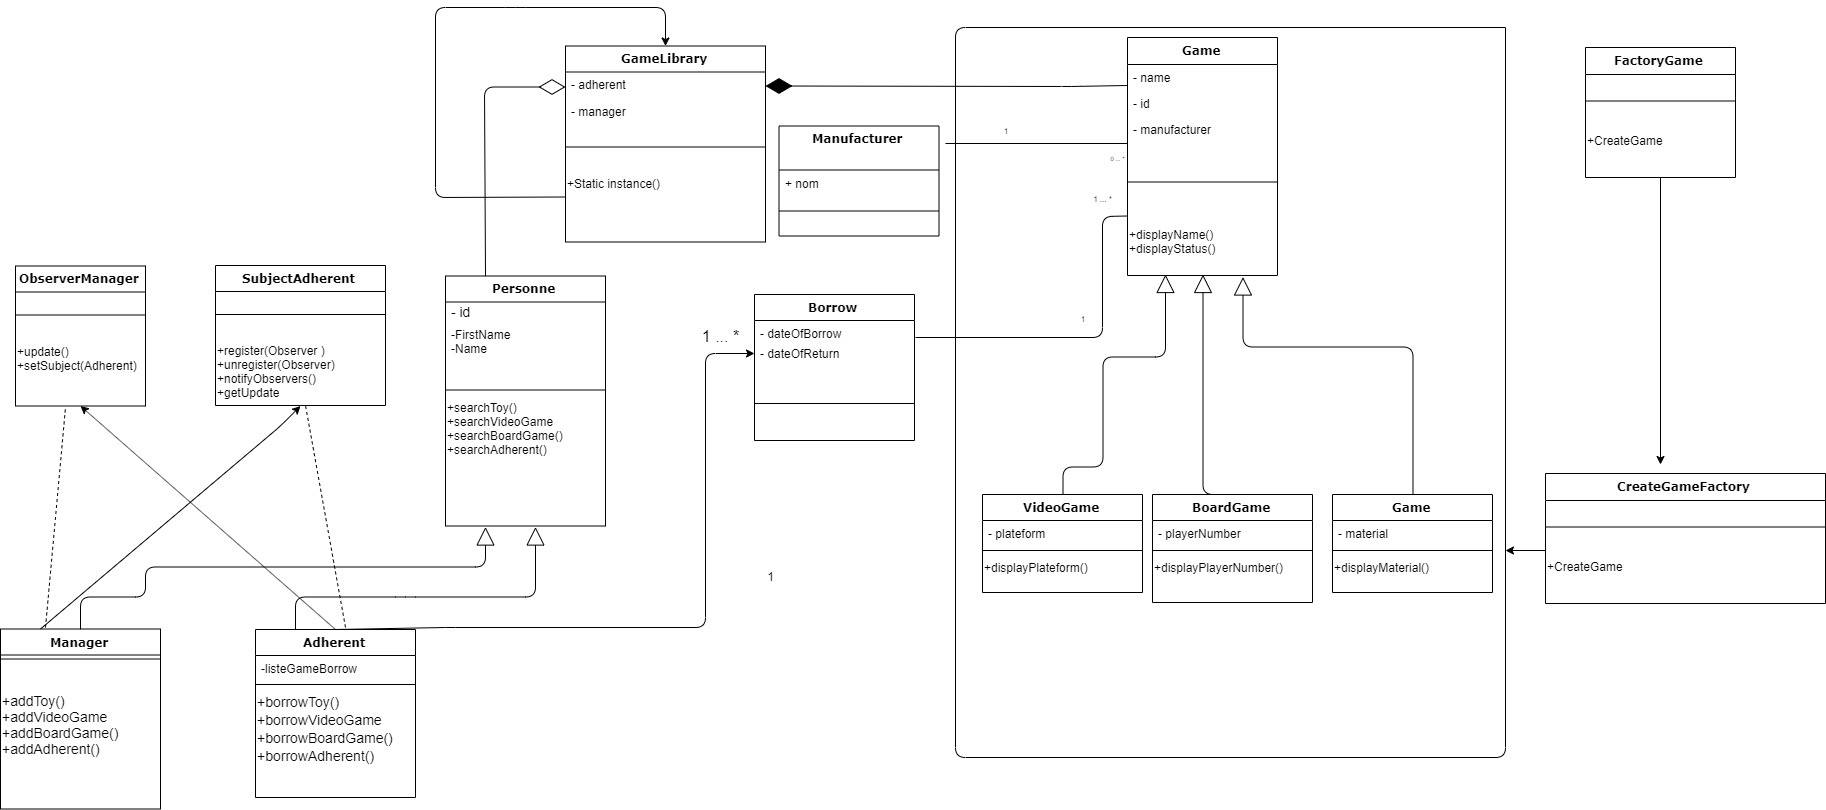
\includegraphics [scale=0.35, angle=90]{Figures/Class_Diagram.jpg}
            \caption{Diagramme de classe}
            \label{fig:annexe:classDiagram_old}
        \end{figure*}